\section{Ανάπτυξη Εφαρμογών}
\label{sec:development}

Η παρούσα παράγραφος περιγράφει την διαδικασία που πρέπει να ακολουθηθεί για να αναπτύξει κάποιος μια εφαρμογή η οποία θα προσαρτηθεί πάνω στον καθρέφτη. Η οργάνωση του συστήματος έχει γίνει με την χρήση των κλάσεων kivy.uix.screenmanager.ScreenManager και kivy.uix.screenmanager.Screen. Τα σημεία που πρέπει να προσέξει κάποιος για να προσαρτήσει την δική του εφαρμογή είναι στην δομή των φακέλων του κώδικα, στην ορθή ανάγνωση του Widget από το λειτουργικό του καθρέφτη, οι σωστή δομή των ρυθμίσεων της προσαρτούμενης εφαρμογής και τέλος οι φωνητικές εντολές που θα είναι διαθέσιμες για τον χρήστη.

\subsection{Δομή Φακέλων}
Η δομή που έχει ο κώδικας του καθρέφτη φαίνεται στο παρακάτω δέντρο.
\\

\dirtree{%
	.1 SmartMirror.
	.2 smartmirror.py.
	.2 smartmirror.kv.
	.2 mirror\_settings.py.
	.2 modules/.
	.3 action.py.
	.3 basedir.py.
	.3 bot.py.
	.3 controller.py.
	.3 speech.py.
	.2 widgets/.
	.3 clock/.
	.3 exercisor/.
	.3 weather/.
}

Οποιαδήποτε καινούργια εφαρμογή αναπτύσει ο χρήστης πρέπει να μπει κάτω από τον φάκελο widgets με την παρακάτω δομή. \\

\dirtree{%
	.1 widgets/.
	.2 <widget\_name>/.
	.3 <widget\_name>.py.
	.3 <widget\_name>.kv.
	.3 settings.json.
}

Με την παραπάνω οργάνωση το λειτουργικό είναι σε θέση να βρει αυτόματα και να προσαρτήσει την εφαρμογή.

\subsection{Εγκατάσταση Οθόνης}
Η γενική οργάνωση του καθρέφτη όσον αφορά την λογική των εξωτερικών εφαρμογών φαίνεται στο Σχήμα \ref{fig:widget_organization}. Η κλάση MainPage είναι ένας ScreenManager ο οποίος διαβάζει όλες τις οθόνες που βρίσκονται στον φάκελο widgets/ και τις προσαρτίζει σε αυτόν.

\begin{figure}[h]
	\centering
	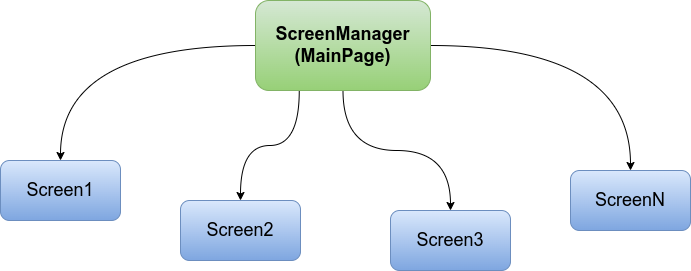
\includegraphics[scale=0.7]{images/chapter4/widget_organization.png}
	\caption{Αναπαράσταση δομής του καθρέφτη}
	\label{fig:widget_organization}
\end{figure}

Προκειμένου να γίνει η προσάρτηση, κάθε widget πρέπει να ορίσει μία συνάρτηση install(manager) η οποία καλεί την εντολή \texttt{manager.add\_widget(<Screen>)}. Κατά την εκκίνηση της εφαρμογής η κλάση MainPage καλεί τις συναρτήσεις install του κάθε widget και έτσι προσθέτει τις συγκεκριμένες οθόνες.

\subsection{Ρυθμίσεις}
